À l'aide de l'étude du déplacement du robot accessible sur le \href{https://gitlab.com/mosee/elech309-2024}{gitlab du projet}, la partie \textit{mouvement} du projet a été scindée en plusieurs étapes :

\begin{enumerate}
    \item[$\bullet$] faire tourner les moteurs à une vitesse donnée
    \item[$\bullet$] déterminer la distance parcourue et la rotation effectuée par le robot
    \item[$\bullet$] générer une consigne acceptable
    \item[$\bullet$] établir un régulateur en translation
    \item[$\bullet$] déterminer les paramètres du régulateur en rotation
    \item[$\bullet$] réécrire le code pour y intégrer ce deuxième régulateur
\end{enumerate}

\section{Moteurs}

Pour alimenter les moteurs, il est nécessaire de leur fournir un signal PWM. Pour générer celui-ci, l'\textit{output compare} est utilisé. Il permet, avec l'aide d'un \textit{timer}, de générer le signal en créneaux désiré.\\ À chaque période du \textit{timer}, il envoie une tension haute à sa sortie jusqu'à ce que le \textit{timer} ait atteint la valeur définie par la variable de configuration \textbf{OCxRS} de l'\textit{output compare} après quoi il sort une tension basse. La fréquence de $20 kHz$ a été choisie pour le \textit{timer} puisqu'il s'agit de la fréquence maximale à laquelle un être humain peut percevoir un son. Cela permet de ne pas entendre de son irrégulier lorsque le moteur tourne. La valeur de seuil du \textit{timer} utilisé est calculée :\\

\begin{align*}
    PR &= \frac{f_{\mu C}}{f_{\text{choisie}}} - 1\\
    &= \frac{40\times10^6}{20\times10^3}-1 = 1999
\end{align*}

Le \textit{timer} "compte" alors jusqu'à $1999$, ce qui veut dire qu'on a une précision de $0.05\%$ sur la commande. Les fonctions \textit{set\_speed\_L} et \textit{set\_speed\_R} (annexe \ref{code:mouvement}) changent donc la valeur de \textbf{OCxRS} et éventuellement le sens de rotation du moteur via le port \textbf{DIRx} du driver.

\begin{figure}[H]
    \centering
    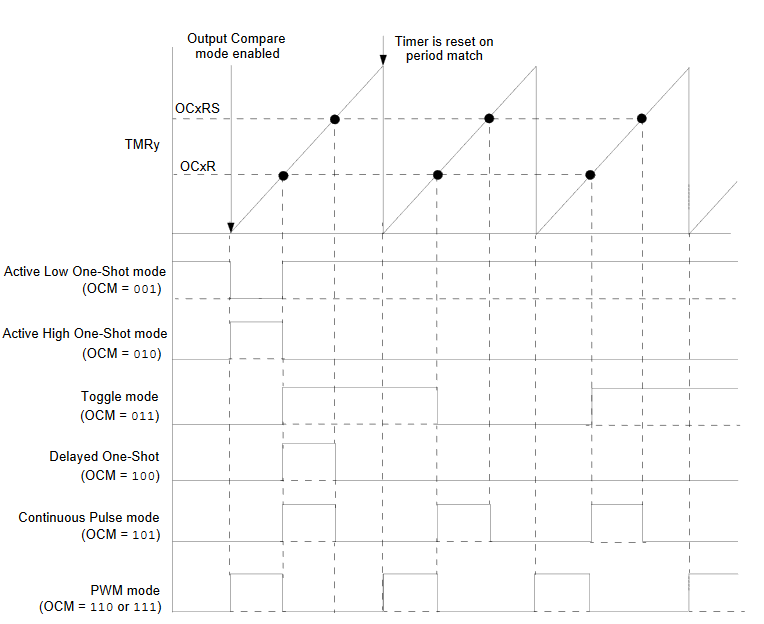
\includegraphics[width=0.9\textwidth]{Pictures/output compare.png}
    \caption{Fonctionnement de l'\textit{output compare}}
    \label{fig:enter-label}
\end{figure}

\section{Mesure de position}

La détermination de la distance parcourue par une roue est déterminée à l'aide du \textit{QEI}. Les roues comptant 360 fentes, un tour complet de roue correspond à une valeur de 1440 dans le registre de sortie du \textit{QEI}, \textbf{POSxCNT} \ref{clk_to_cm}. Puisque la valeur de ce registre est susceptible d'atteindre des grandes valeurs tant positives que négatives, \textit{POSxCNT} est remis à $0x8000$ (la moitié d'un stockage à $16$ bits) avant chaque exécution de commande évitant ainsi les \textit{underflow} ou les \textit{overflow}. Pour la régulation en rotation, on passe de la distance à l'angle grâce à \ref{cm_to_ang}.

\begin{equation}
    d = \frac{POSxCNT \times 2 \times \pi}{1440}
    \label{clk_to_cm}
\end{equation}
\begin{equation}
    \alpha = \frac{d \times 180}{E \times \pi}
    \label{cm_to_ang}
\end{equation}

Où $d$ est la distance parcourue, $\alpha$ l'angle effectué par le robot et $E$ son empatement.

\section{Génération de consigne}
\label{chap:consigne}
Il a été choisi de calculer à l'avance la position du robot lors de la phase d'accélération et de décélération sans stocker la position désirée lors du MRU (voir fig \ref{consigne}). Ceci permet d'avoir une liste de positions dont la taille est fixée par l'accélération et la vitesse maximale puisque le temps total sera égal à $2\frac{v_{max}}{a}$. Pour réduire le nombre de calculs nécessaires, la seconde partie de la consigne n'est que la distance finale à laquelle on soustrait le début de la consigne. On ajoute aussi à la fin de la liste de commande la distance finale pendant 15 centièmes de seconde pour être certain que le robot ait atteint son objectif avant de s'arrêter.

\begin{figure}[H]
    \centering
    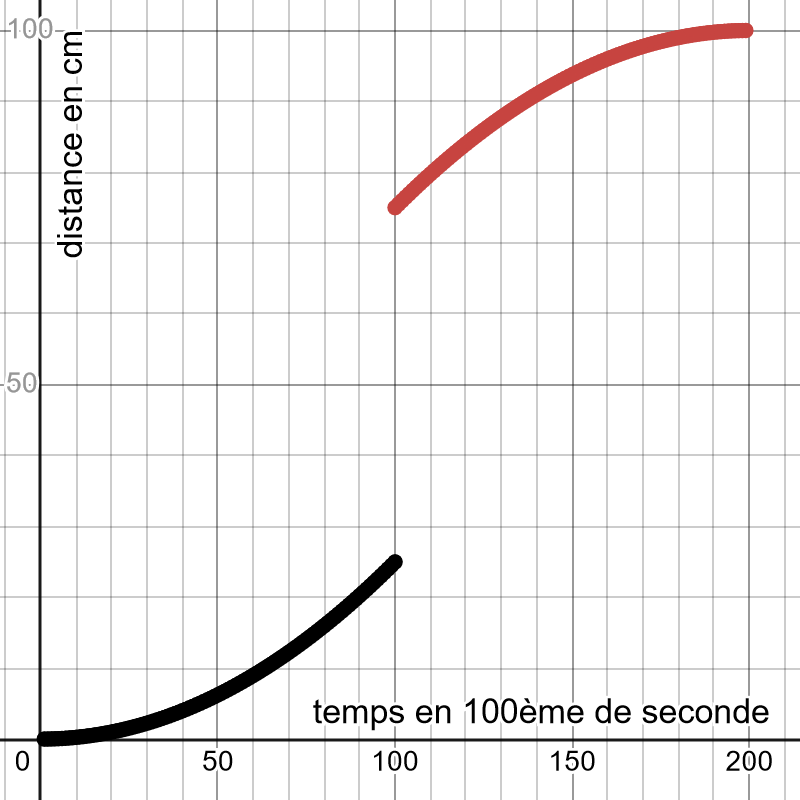
\includegraphics[width=0.9\textwidth]{Pictures/consigne.png}
    \caption{consigne pour une translation de 100 cm}
    \label{consigne}
\end{figure}

\section{Régulateur en translation}

La mise en place du régulateur est facilement réalisable à partir du schéma fonctionnel (fig : \ref{fig:regulateur_translation}). La première difficulté rencontrée a été de régler le \textit{timer} pour qu'il fonctionne à $100Hz$. Puisqu'avec la fréquence de fonctionnement du dsPIC $f_{\mu C} = 40\times10^6 Hz$, il aurait fallu qu'il compte jusqu'à $\frac{40\times10^6}{100}-1 = 399999$, or la valeur de réglage du \textit{timer} est sur 16 bits donc on ne peut pas dépasser $2^{16} = 65536$. on a donc pris $PR = 57143$ et on n'utilise le régulateur qu'après que le \textit{timer} ait "sonné" 7 fois.

\begin{figure}[H]
    \centering
    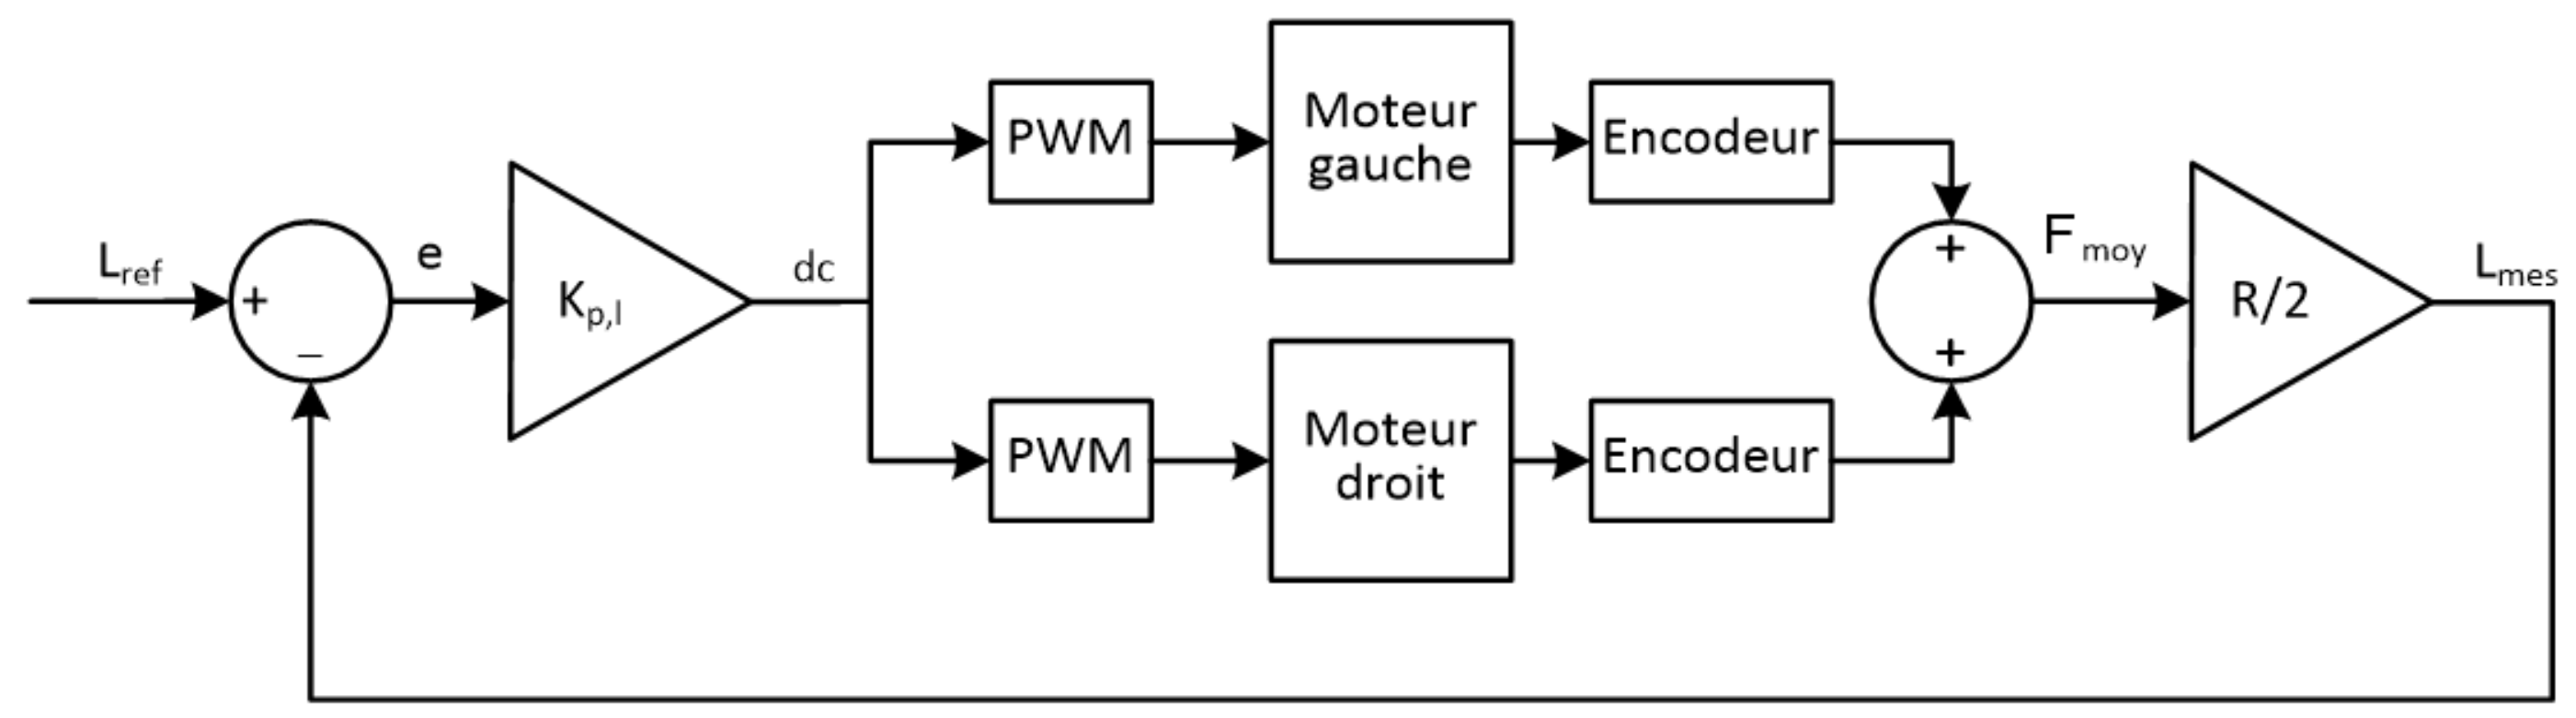
\includegraphics[width=0.9\textwidth]{Pictures/regul_trans.png}
    \caption{Fonctionnement du \textit{Régulateur en translation}}
    \label{fig:regulateur_translation}
\end{figure}

L'autre point complexe a été qu'il n'y a pas de consigne pour la phase à laquelle le robot est à vitesse constante (comme expliqué \ref{chap:consigne}). La commande envoyée au moteur n'est donc pas modifiée pendant tout le temps où le robot est en MRU. Pour savoir quand se remettre à suivre la consigne, le microcontrôleur compare son ancienne commande de vitesse avec celle qu'il devrait appliquer si la consigne était celle du début de la décélération (en valeur absolue). Si la nouvelle commande est inférieure à l'ancienne, il reprend sa régulation en MRUA.\\
Comme on peut le voir dans le code (annexe \ref{code:mouvement}), la variable \textit{t} sert de temps. Elle est utilisée pour savoir à quelle valeur de la consigne on est censé être et elle est incrémentée à chaque fois que la commande est modifiée. Quand la phase d'accélération est terminée, on arrête d'incrémenter \textit{t} tous les centièmes de secondes. On recommence à augmenter \textit{t} quand le robot arrive dans sa phase de décélération.

\section{Régulateur en rotation}

\subsection{Modélisation du robot en rotation}

Tout comme pour la régulation en translation, il faut déterminer le modèle du robot en rotation pour dimensionner le régulateur proportionnel. Pour ce faire, on mène une série d'expériences (identiques à celles de la régulation en translation) dont les résultats sont affichés sur les figures \ref{fig:statrot} \& \ref{fig:approxrot}

\begin{figure}[H]
    \centering
    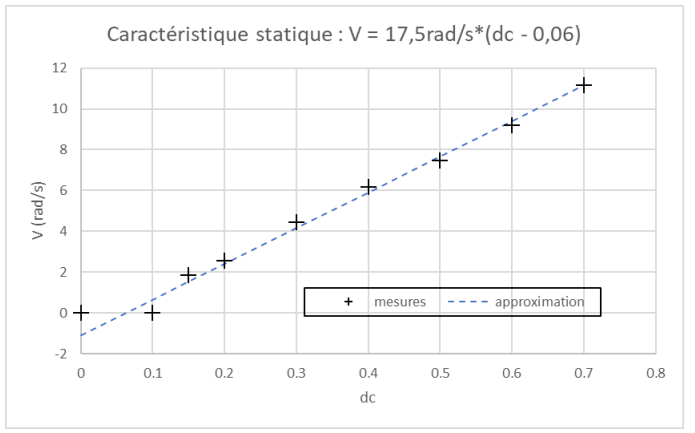
\includegraphics[width=0.9\textwidth]{Pictures/caracstatrot.png}
    \caption{Caractéristique statique en rotation}
    \label{fig:statrot}
\end{figure}

\begin{figure}[H]
    \centering
    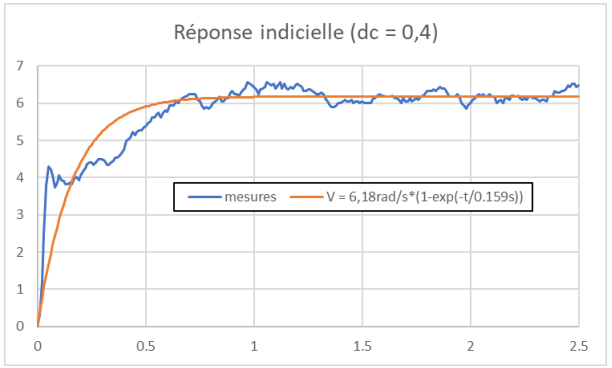
\includegraphics[width=0.9\textwidth]{Pictures/approxreponstati.png}
    \caption{Approximation de la réponse indicielle pour dc=0.3}
    \label{fig:approxrot}
\end{figure}

On peut modéliser le robot en rotation par la fonction de transfert suivante, qui est identique dans la forme à celle du robot en translation : 
\begin{align*}
H_r(p)&=\frac{V(p)}{U(p)}=\frac{k_r}{(1+p \tau)} \frac{1}{p}
\end{align*}

La pente de la droite sur la caractéristique statique sur la figure \ref{fig:statrot} donne la valeur de $k_r$ et la constante de temps dans l'approximation de la réponse indicielle sur la figure \ref{fig:approxrot} donne la valeur de $\tau$. On peut donc réécrire la fonction de transfert de la manière suivante :

\begin{align*}
H_r(p)&=\frac{17.5}{(1+0.159p )} \frac{1}{p}
\end{align*}

Le schéma de régulation est représentée sur la figure \ref{fig:schémaregrot}. Sachant que la période d'échantillonnage vaut $\frac{1}{100 \ Hz}$, il ne reste plus que le gain $k_p$ à déterminer.

\begin{figure}[H]
    \centering
    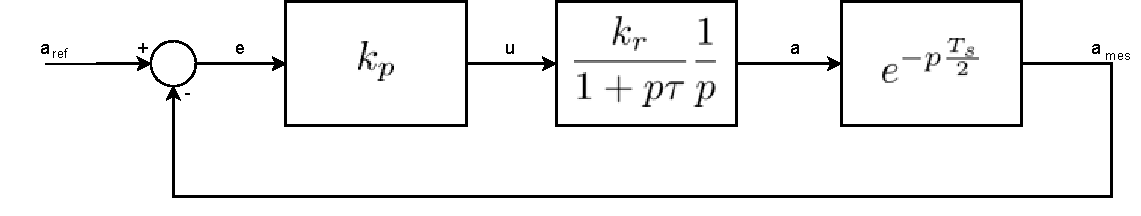
\includegraphics[width=0.9\textwidth]{pdffiles/regrot.drawio.pdf}
    \caption{Schéma de régulation en rotation}
    \label{fig:schémaregrot}
\end{figure}

\subsection{Dimensionnement du régulateur en rotation}

Le dimensionnement du régulateur se fait à partir des critères des marges de gain et de phase. Ces marges sont identiques à celles évoquées dans la régulation en translation puisque les modèles des 2 régulateurs sont similaires.

\subsubsection{Marge de gain}

L'expression du gain est : 

\begin{align*}
    k_{p1} &= \frac{\omega_1 \sqrt{1 +(\omega_1 \tau)^2 }}{2 k_r}
\end{align*}

Où on a besoin de trouver la valeur de $\omega_1$. On peut la déduire à partir de l'équation suivante :

\begin{align*}
    \text{Atan}(\omega_1 \tau)+ \omega_1 \frac{T_s }{2}=\frac{\pi}{2} 
\end{align*}

A l'aide du site internet \url{https://www.geogebra.org/calculator}, on trouve graphiquement la valeur de $\omega_1$ sur la figure \ref{fig:omega1} et elle vaut $35.28 \ rad/s$.

\begin{figure}[H]
    \centering
    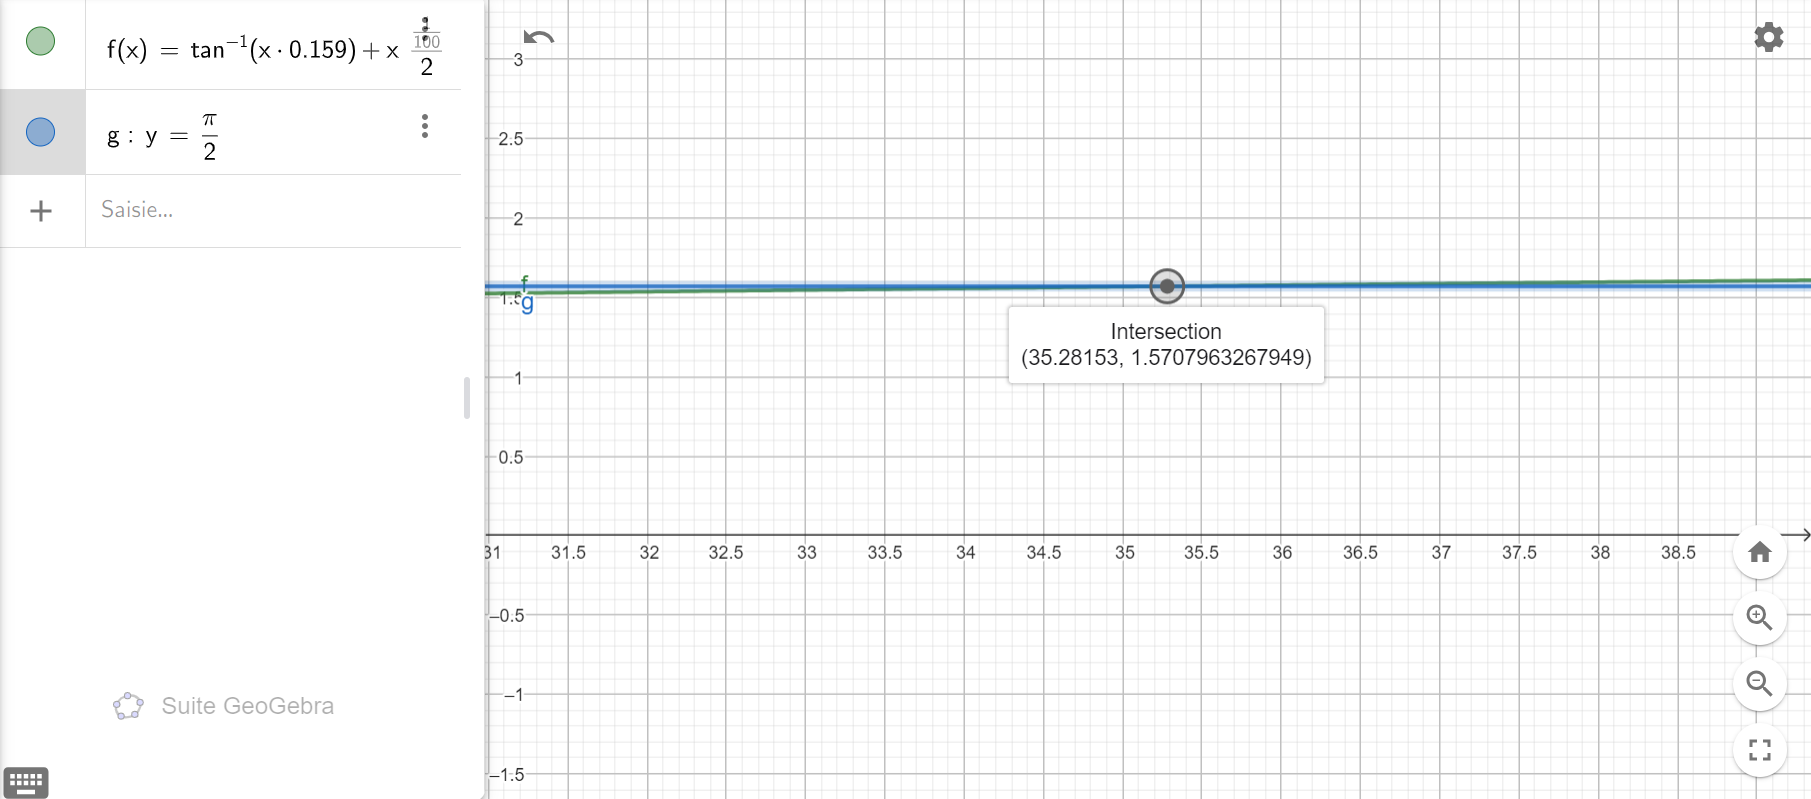
\includegraphics[width=0.9\textwidth]{Pictures/omega_1_marge_gain.png}
    \caption{Résolution graphique pour déterminer $\omega_1$}
    \label{fig:omega1}
\end{figure}

Ainsi, on peut calculer la valeur de $k_{p1}$ :

\begin{align*}
     k_{p1} &= \frac{35.28 \sqrt{1 +(35.28 \cdot 0.159)^2 }}{2 \cdot 17.5} \\
     &= 5.74354 \ rad^{-1}
\end{align*}

\subsubsection{Marge de phase}

L'expression du gain est : 

\begin{align*}
    k_{p2} &= \frac{\omega_2 \sqrt{1 +(\omega_2 \tau)^2 }}{ k_r}
\end{align*}

On a besoin de trouver la valeur de $\omega_2$. On peut la déduire à partir de l'équation suivante :

\begin{align*}
    arctg(\omega_2 \tau)+ \omega_1 \frac{T_s }{2}=\frac{\pi}{3} 
\end{align*}

Comme avant, on trouve graphiquement la valeur de $\omega_2$ sur la figure \ref{fig:omega2} et elle vaut $9.7605 \ rad/s$.

\begin{figure}[H]
    \centering
    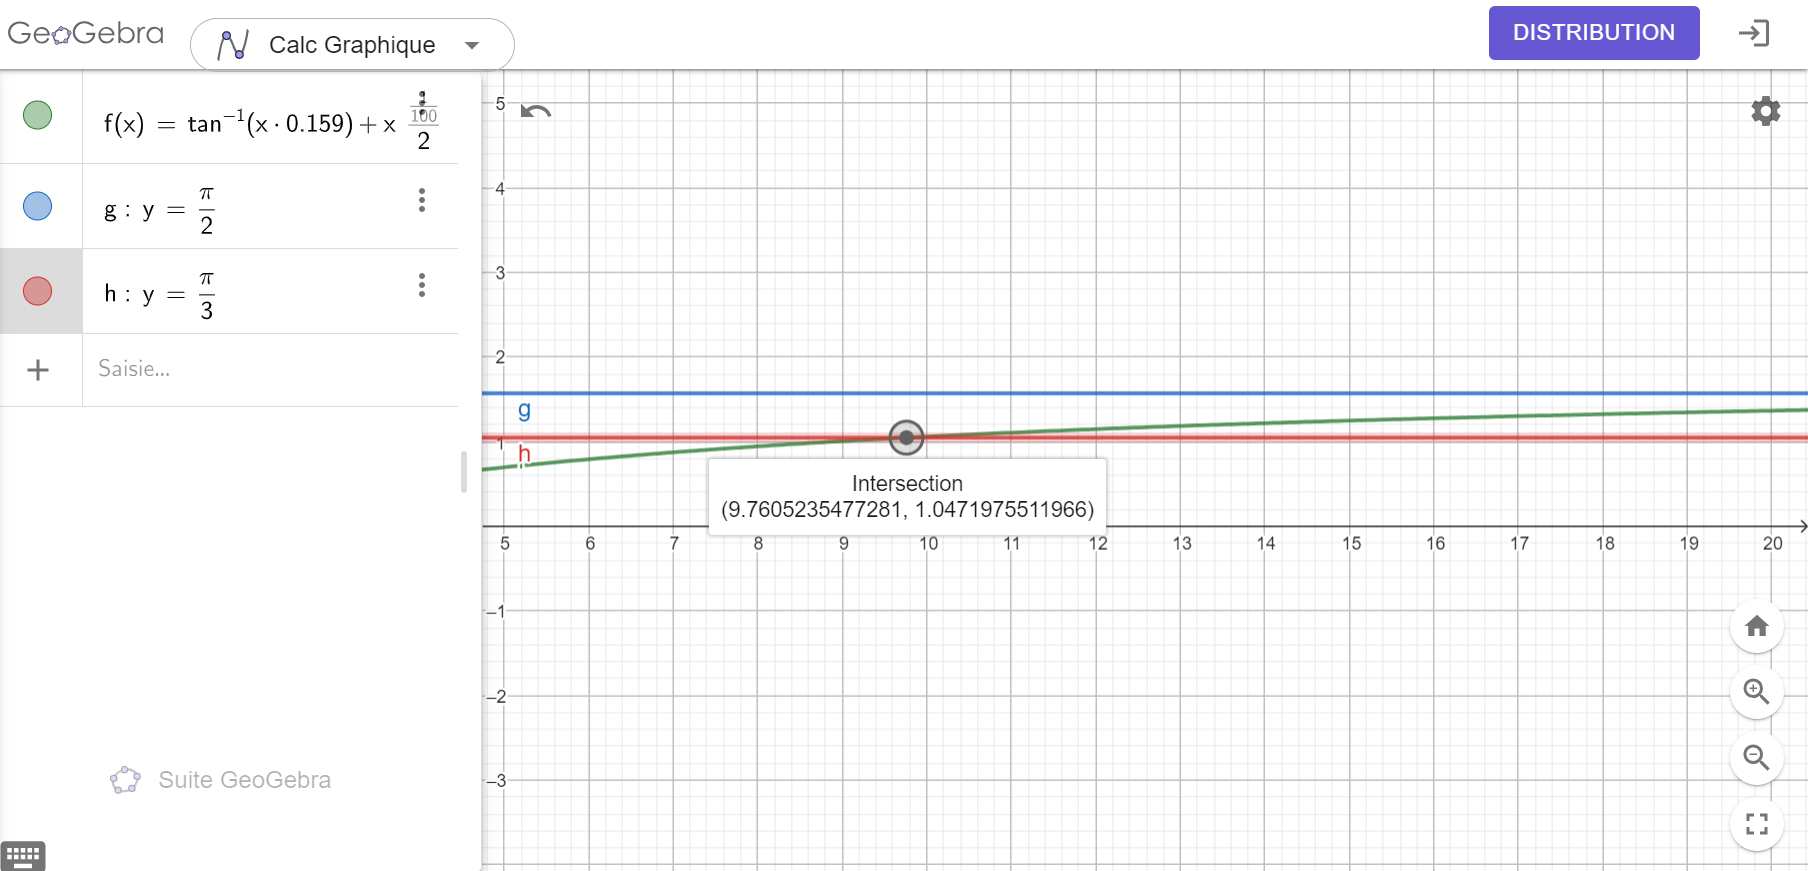
\includegraphics[width=0.9\textwidth]{Pictures/omega_2_marge_phase.png}
    \caption{Résolution graphique pour déterminer $\omega_2$}
    \label{fig:omega2}
\end{figure}

Ainsi, on peut calculer la valeur de $k_{p2}$ :

\begin{align*}
     k_{p1} &= \frac{9.7605 \sqrt{1 +(9.7605 \cdot 0.159)^2 }}{ 17.5} \\
     &= 1.0297\ rad^{-1}
\end{align*}

\subsubsection{Valeur finale du gain}

Il faut choisir le plus petit gain et il s'agit de $k_{p2}$. Cependant puisqu'on travaille en degré, il faut changer les unités du gain :
\begin{align*}
     k_{p1} &= 1.0297\ rad^{-1} \\
     &= 0.017971 \ \text{°}^{-1}
\end{align*}


\section{Régulateur complet}

La génération de consigne a simplement demandé l'ajout d'une liste contenant les commandes en rotation. Sur base du schéma en bloc donné sur \href{https://gitlab.com/mosee/elech309-2024}{gitlab}, le code a été modifié afin d'inclure les 2 régulateurs.

\begin{figure}[H]
    \centering
    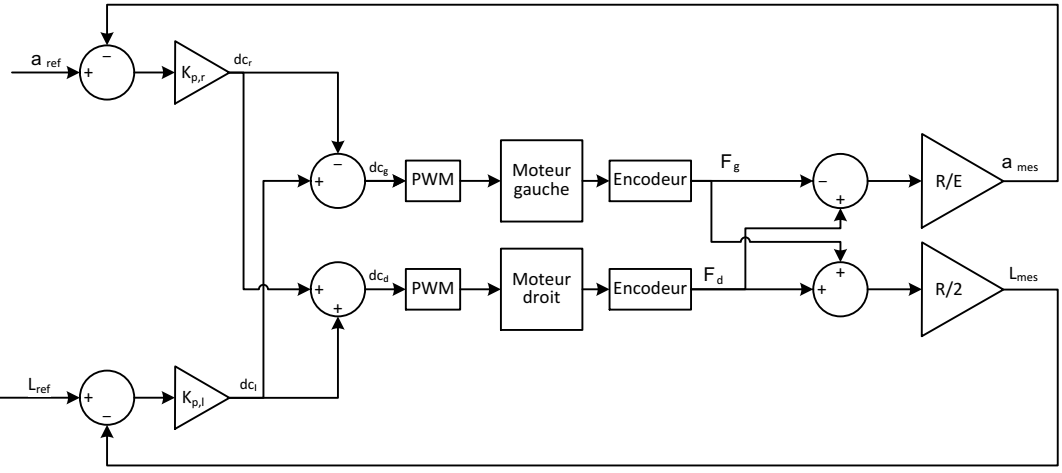
\includegraphics[width=0.9\textwidth]{Pictures/regul_pol.png}
    \caption{Fonctionnement du \textit{Régulateur en translation}}
    \label{fig:enter-label}
\end{figure}

La plus importante des modifications à effectuer a été d'ajouter un régulateur en MRU là où la consigne n'était pas modifiée précédemment, de manière à empêcher le robot de tourner en ligne droite ou d'avancer lors d'une rotation.

\section{Vérification du code}

Certaines sections du code ont été légèrement modifiées pour s'exécuter sur un ordinateur, de façon à vérifier leur bon fonctionnement. Dans cette partie qui ne s'intéresse qu'au mouvement, la seule fonction qui est implémentable est la génération de consigne, qui est en annexe (\ref{code:test_consigne}) et qui a permis de s'assurer que les listes de positions et d'angles soient correctes quelle que soit la commande.
